\documentclass{article}
\usepackage[UTF8]{ctex}
\usepackage[T1]{fontenc}
\usepackage[utf8]{inputenc}
\usepackage[colorlinks, linkcolor = black]{hyperref}
\usepackage{latexsym}
\usepackage{amsmath}
\usepackage{geometry}
\usepackage{ulem}
\usepackage{xcolor}
\usepackage{amsthm}
\usepackage{enumerate}
\usepackage{enumitem}
\usepackage{amssymb}
\usepackage{tikz}
\usetikzlibrary{calc}
\usetikzlibrary{positioning}
\usetikzlibrary{arrows}

\newcounter{BPTnodes}
\newcommand{\BPnode}[4]{
    \stepcounter{BPTnodes}
    \node[rectangle, draw, black, minimum width = 1.6em, minimum height = 1.6em, inner sep = 2pt] (\theBPTnodes D1) at (#1) {#2};
    \node[rectangle, draw, black, minimum width = 1.6em, minimum height = 1.6em, inner sep = 2pt] (\theBPTnodes D2) [right = 0em of \theBPTnodes D1]{#3};
    \node[rectangle, draw, black, minimum width = 1.6em, minimum height = 1.6em, inner sep = 2pt] (\theBPTnodes D3) [right = 0em of \theBPTnodes D2]{#4};
    \node[rectangle, draw, black, minimum width = 1.2em, minimum height = 1.6em, inner sep = 2pt] (\theBPTnodes P1) [below left = 0em and -1.2em of \theBPTnodes D1] {};
    \node[rectangle, draw, black, minimum width = 1.2em, minimum height = 1.6em, inner sep = 2pt] (\theBPTnodes P2) [right = 0em of \theBPTnodes P1] {};
    \node[rectangle, draw, black, minimum width = 1.2em, minimum height = 1.6em, inner sep = 2pt] (\theBPTnodes P3) [right = 0em of \theBPTnodes P2] {};
    \node[rectangle, draw, black, minimum width = 1.2em, minimum height = 1.6em, inner sep = 2pt] (\theBPTnodes P4) [right = 0em of \theBPTnodes P3] {};
    % \coordinate (\theBPTnodes head) at ($(\theBPTnodes D1) - (1.4em, 1.4em)$);
    % \coordinate (\theBPTnodes tail) at ($(\theBPTnodes P4) + (1.05em, 1.4em)$);
    % \draw [draw = black] (\theBPTnodes head) rectangle (\theBPTnodes tail);
    % \coordinate (\theBPTnodes) at ($(\theBPTnodes D2) + (0, 0.7em)$);
    \coordinate ({\theBPTnodes}Point1) at ($(\theBPTnodes P1)$);
    \coordinate ({\theBPTnodes}Point2) at ($(\theBPTnodes P2)$);
    \coordinate ({\theBPTnodes}Point3) at ($(\theBPTnodes P3)$);
    \coordinate ({\theBPTnodes}Point4) at ($(\theBPTnodes P4)$);

}

\setlist{
    leftmargin = .1\linewidth,
    % rightmargin = .1\linewidth,
    % label=\emph{\alph*}.
}

\geometry{left = 2cm, right = 2cm}
\makeatletter
\renewcommand{\section}{\@startsection{section}{1}{0mm}
                                {-5ex plus -.5ex minus -.2ex}
                                {3ex plus .2ex}
                                {\normalfont\large\bfseries}}
\makeatother
\title{Homework 6}
\author{PB17000297 罗晏宸}
\date{April 26 2020}

\begin{document}
\maketitle

\section{考虑下面的 B+ 树(n = 3):}
\begin{figure}[h]
    \centering
    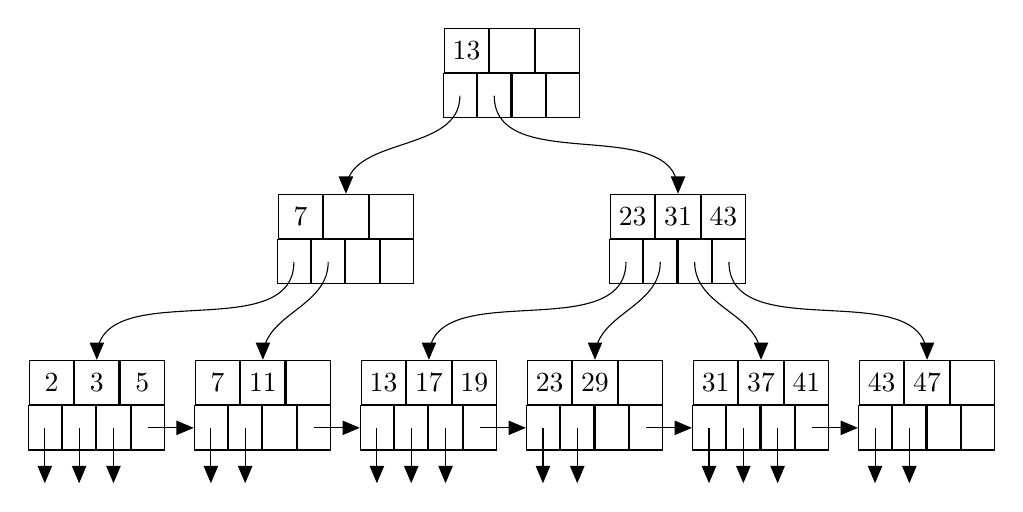
\begin{tikzpicture}[arrows = {-triangle 45}]
        \BPnode{0, 0}{13}{}{}
        \BPnode{-6em, -6em}{7}{}{}
        \BPnode{6em, -6em}{23}{31}{43}
        \BPnode{-15em, -12em}{2}{3}{5}
        \BPnode{-9em, -12em}{7}{11}{}
        \BPnode{-3em, -12em}{13}{17}{19}
        \BPnode{3em, -12em}{23}{29}{}
        \BPnode{9em, -12em}{31}{37}{41}
        \BPnode{15em, -12em}{43}{47}{}
        \draw[] ({1}Point1) to[out = -90, in = 90] (2D2);
        \draw[] ({1}Point2) to[out = -90, in = 90] (3D2);
        \draw[] ({2}Point1) to[out = -90, in = 90] (4D2);
        \draw[] ({2}Point2) to[out = -90, in = 90] (5D2);
        \draw[] ({3}Point1) to[out = -90, in = 90] (6D2);
        \draw[] ({3}Point2) to[out = -90, in = 90] (7D2);
        \draw[] ({3}Point3) to[out = -90, in = 90] (8D2);
        \draw[] ({3}Point4) to[out = -90, in = 90] (9D2);
        \draw[] ({4}Point1) to ($({4}Point1) - (0, 2.0em)$);
        \draw[] ({4}Point2) to ($({4}Point2) - (0, 2.0em)$);
        \draw[] ({4}Point3) to ($({4}Point3) - (0, 2.0em)$);
        \draw[] ({4}Point4) to (5P1);
        \draw[] ({5}Point1) to ($({5}Point1) - (0, 2.0em)$);
        \draw[] ({5}Point2) to ($({5}Point2) - (0, 2.0em)$);
        \draw[] ({5}Point4) to (6P1);
        \draw[] ({6}Point1) to ($({6}Point1) - (0, 2.0em)$);
        \draw[] ({6}Point2) to ($({6}Point2) - (0, 2.0em)$);
        \draw[] ({6}Point3) to ($({6}Point3) - (0, 2.0em)$);
        \draw[] ({6}Point4) to (7P1);
        \draw[] ({7}Point1) to ($({7}Point1) - (0, 2.0em)$);
        \draw[] ({7}Point2) to ($({7}Point2) - (0, 2.0em)$);
        \draw[] ({7}Point4) to (8P1);
        \draw[] ({8}Point1) to ($({8}Point1) - (0, 2.0em)$);
        \draw[] ({8}Point2) to ($({8}Point2) - (0, 2.0em)$);
        \draw[] ({8}Point3) to ($({8}Point3) - (0, 2.0em)$);
        \draw[] ({8}Point4) to (9P1);
        \draw[] ({9}Point1) to ($({9}Point1) - (0, 2.0em)$);
        \draw[] ({9}Point2) to ($({9}Point2) - (0, 2.0em)$);
    \end{tikzpicture}
    \label{B+}
\end{figure}
\subparagraph{1)} 画出依次插入了 36, 18, 40 后的 B+ 树;
\subparagraph{2)} 画出在 1) 所得的 B+ 树中依次删除 43, 13, 7 之后最终的 B+ 树

\paragraph{解}

\section{假设有如下的键值,现用 5 位二进制序列来表示每个键值的 hash 值。回答问题:}
\begin{table}[h]
    \centering
    \begin{tabular}{ccccccc}
        A [11001] & B [00111] & C [00101] & D [00110] & E [10100] & F [01000] & G [00011] \\
        H [11110] & I [10001] & J [01101] & K [10101] & L [11100] & M [01100] & N [11111]
    \end{tabular}
\end{table}
\subparagraph{1)} 如果将上述键值按 A 到 N 的顺序插入到可扩展散列索引中,若每个桶大小为一个磁盘块,每个磁盘块最多可容纳 3 个键值,且初始时散列索引为空,则全部键值插入完成后该散列索引中共有几个桶?并请写出键值 E 所在的桶中的全部键值。
\subparagraph{2)} 前一问题中,如果换成线性散列索引,其余假设不变,同时假设只有当插入新键值后空间利用率大于 80\%时才增加新的桶,则全部键值按序插入完成后该散列索引中共有几个桶?并请写出键值 B 所在的桶中的全部键值(包括溢出块中的键值)。
\end{document}
